\documentclass{standalone}
\usepackage{pgf,tikz}

\begin{document}

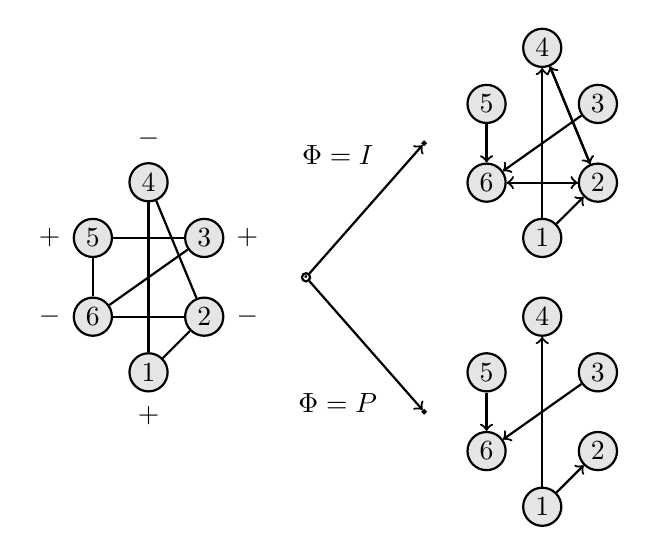
\begin{tikzpicture}
   [scale=0.5,every node/.style={circle, thick, draw=black,fill=black!10,inner sep=2pt}]

  \node[label=below:$+$] (n1) at (0,0)  		{$1$};
  \node[label=right:$-$] (n2) at (1.414,1.414)  {$2$};
  \node[label=right:$+$] (n3) at (1.414,3.414)  {$3$};
  \node[label=above:$-$] (n4) at (0,4.828)  	{$4$};
  \node[label=left:$+$] (n5) at (-1.414,3.414) {$5$};
  \node[label=left:$-$] (n6) at (-1.414,1.414) {$6$};

  \node(n1i) at (10,3.414) {$1$};
  \node(n2i) at (11.414,4.818) {$2$};
  \node(n3i) at (11.414,6.818) {$3$};
  \node(n4i) at (10,8.242) {$4$};
  \node(n5i) at (8.586,6.818) {$5$};
  \node(n6i) at (8.586,4.818) {$6$};

  \node(n1p) at (10,-3.414) {$1$};
  \node(n2p) at (11.414,-2) {$2$};
  \node(n3p) at (11.414,0) {$3$};
  \node(n4p) at (10,1.414) {$4$};
  \node(n5p) at (8.586,0) {$5$};
  \node(n6p) at (8.586,-2) {$6$};

  \node[fill=white,inner sep=0pt](tr) at (4,2.414) {.};
  \node[fill=white,inner sep=0pt](tri) at (7,5.818) {};
  \node[fill=white,inner sep=0pt](trp) at (7,-1) {};


  \foreach \from/\to in {n1/n2,n1/n4,n2/n4,n5/n3,n5/n6,n6/n3,n2/n6}
    \draw[thick] (\from) -- (\to);

   \foreach \fromi/\toi in {n1i/n2i,n1i/n4i,n3i/n6i,n5i/n6i,n2i/n4i,n4i/n2i,n2i/n6i,n6i/n2i}
   	\draw[->, thick]  (\fromi) -- (\toi);
   	
   \foreach \fromp/\top in {n1p/n2p,n1p/n4p,n3p/n6p,n5p/n6p}
   	\draw[->, thick]  (\fromp) -- (\top);
   	
   	\draw[->, thick] (tr) --  (tri) node [draw = none, near start, above=15pt, fill=white] {$\Phi=I$};
   	\draw[->, thick] (tr) --  (trp) node [draw = none, near start, below=15pt, fill=white] {$\Phi=P$};
 	
\end{tikzpicture}

\end{document}
